\documentclass[11pt,a4paper]{article}

\usepackage[margin=25mm]{geometry}
\usepackage{amsmath,amssymb}
\usepackage{booktabs}
\usepackage{graphicx}
\usepackage{microtype}
\usepackage{xcolor}
\usepackage[hidelinks]{hyperref}

\graphicspath{{../all_on/plot/}{../model/plot/}}
\setlength{\parindent}{0pt}
\setlength{\parskip}{0.65em}

\newcommand{\Prob}{\mathbb{P}}
\title{Customer Load Violation Model\\\large Current Findings}
\author{}
\date{21 September 2026}

\begin{document}
\maketitle

\section{Mathematical formulation}

N numbers of customers are divided into small (S), medium (M), and large (L) classes.  Let
\(n_S,n_M,n_L\) denote the number of customers in each class and let
\(I_S,I_M,I_L\) denote their respective current demands.  This means: 
\begin{equation}
    n_S+n_M+n_L=N, \qquad n_S,n_M,n_L\in\{0,1,\ldots,N\}.
\end{equation}
And for customer \(i\) in class \(j\in\{S,M,L\}\), define the state
\(X_{j,i}\in\{0,1\}\), where 1 means on and 0 means off.  The aggregate current is:
\begin{equation}
    A=\sum_{j\in\{S,M,L\}} I_j\sum_{i=1}^{n_j}X_{j,i}.
\end{equation}
A violation occurs when the aggregate current is strictly above the network
limit \(T\).  Its probability is:
\begin{equation}
    \Prob(A>T).
\end{equation}
The current study uses:
\begin{equation}
    (I_S,I_M,I_L)=(20,40,100),\qquad N=40,\qquad T=1000.
\end{equation}


\section{All-On model}

Assuming all customer loads are on, every state variable is fixed at
\(X_{j,i}=1\), so the aggregate current for a given composition is:
\begin{equation}
    A_{\mathrm{all}}=I_Sn_S+I_Mn_M+I_Ln_L.
\end{equation}
Consequently, the violation probability for a fixed composition is
\begin{equation}
    \Prob(A>T\mid n_S,n_M,n_L,\text{all on})=
    \begin{cases}
        1, & I_Sn_S+I_Mn_M+I_Ln_L>T,\\
        0, & I_Sn_S+I_Mn_M+I_Ln_L\leq T.
    \end{cases}
\end{equation}


The graph demonstrates the violating and non-violating composition
points for the parameters \(I_S=20\), \(I_M=40\), \(I_L=100\), \(N=40\), and
\(T=1000\).

\begin{figure}[htbp]
    \centering
    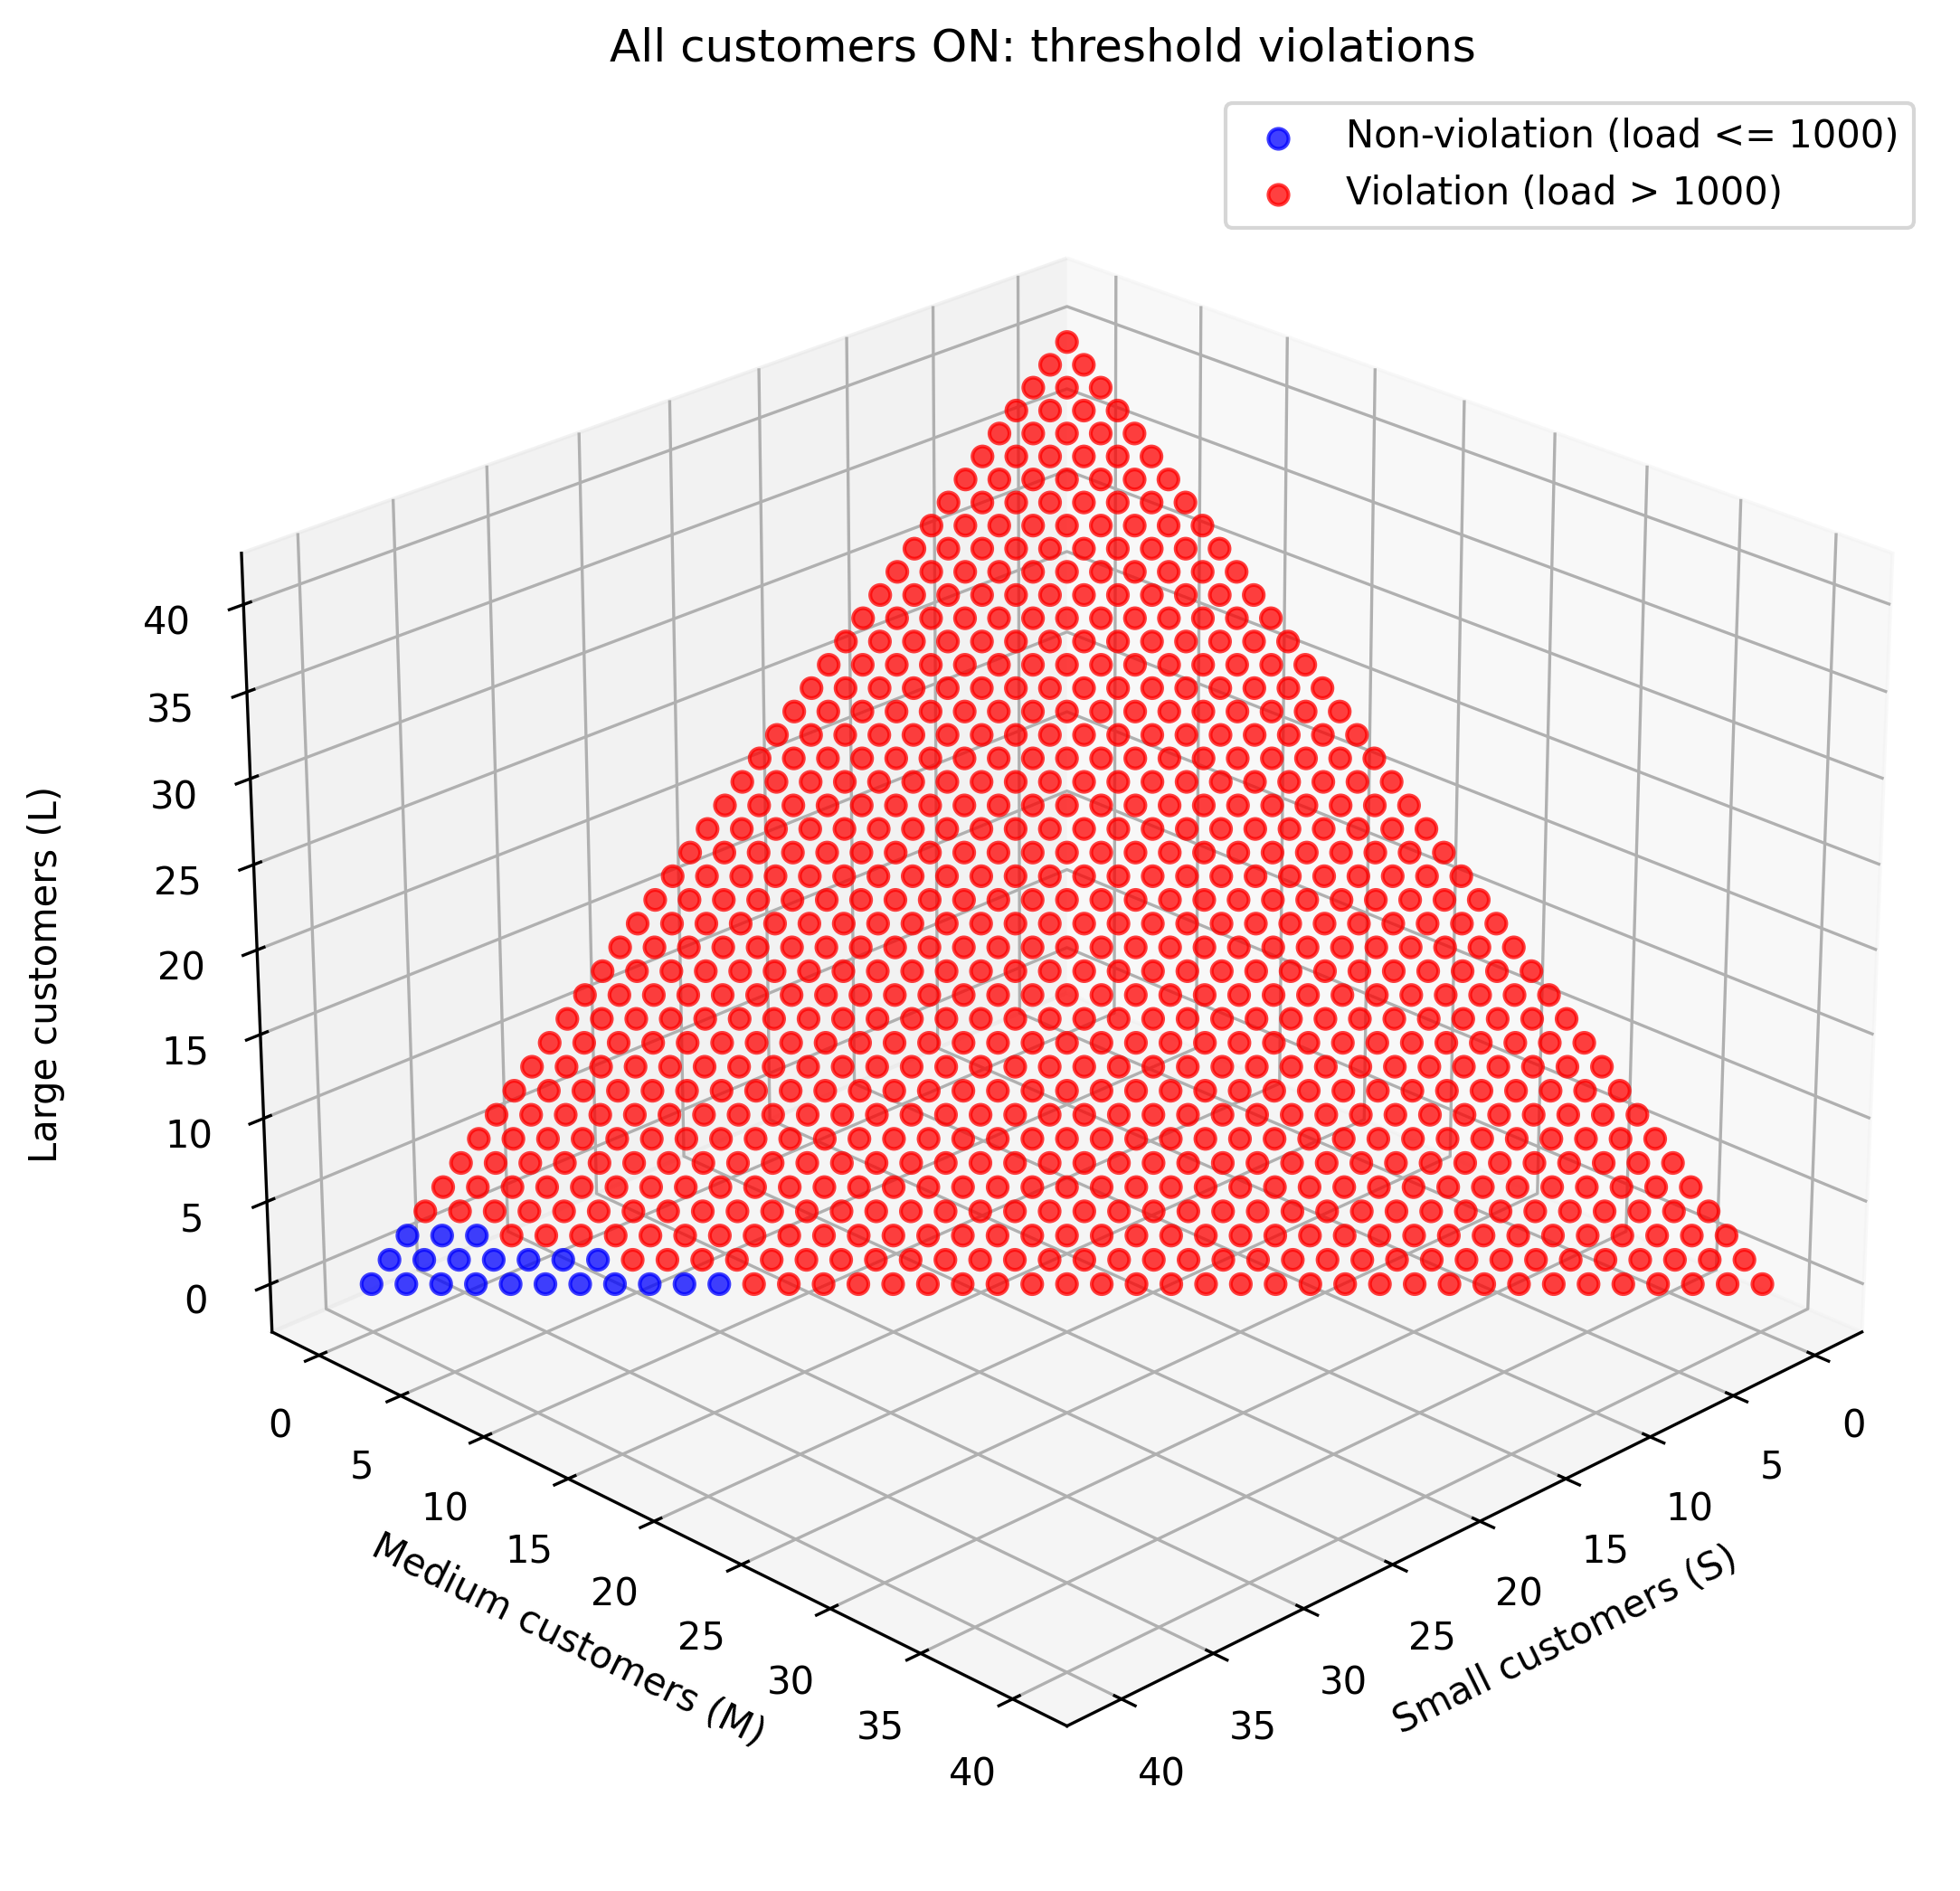
\includegraphics[width=0.82\textwidth]{violations_3d.png}
    \caption{All-On model results.}
    \label{fig:all-on}
\end{figure}

To count the total number of compositions, each composition corresponds to a different placement of the two separators in the array:
\[
    \underbrace{\star\cdots\star}_{n_S}
    \quad\big|\quad
    \underbrace{\star\cdots\star}_{n_M}
    \quad\big|\quad
    \underbrace{\star\cdots\star}_{n_L}
    \qquad .
\]
Choosing the two separator positions among \(N+2\) positions gives
\begin{equation}
    \text{Number of compositions}=\binom{N+2}{2}
    =\frac{(N+2)(N+1)}{2}.
\end{equation}
Empty groups are allowed.  For \(N=40\), this gives
\(\binom{42}{2}=861\) compositions.
The model finds 840 violating compositions.  
\begin{equation}
    \Prob(A>T\mid\text{uniform composition, all on})
    =\frac{840}{861}=0.9756\quad (97.56\%).
\end{equation}

\section{On--Off model}

The On-Off model treats customers as independent Bernoulli loads.  In the
current run,
\begin{equation}
    X_{j,i}\overset{\mathrm{ind}}{\sim}\operatorname{Bernoulli}(p),
    \qquad p=0.5.
\end{equation}
For each class \(j\), define \(Y_j\) as the number of active customers in that
class.  It is the sum of the individual on--off states and therefore has a
binomial distribution:
\begin{equation}
    Y_j=\sum_{i=1}^{n_j}X_{j,i}\sim\operatorname{Binomial}(n_j,p),
    \qquad j\in\{S,M,L\}.
\end{equation}
The random aggregate current in one trial is then
\begin{equation}
    A=I_SY_S+I_MY_M+I_LY_L.
\end{equation}



The implemented model estimates the probability of violations by Monte
Carlo simulation.  For each of the 861 feasible compositions, it performs the
following calculation independently:
\begin{enumerate}
    \item draw \(Y_S,Y_M,Y_L\) from their binomial distributions;
    \item calculate \(A=I_SY_S+I_MY_M+I_LY_L\);
    \item record whether \(A>T\); and
    \item run 100,000 trials for each of five seeds (42--46), giving
    \(N_{\mathrm{trials}}=500{,}000\) pooled trials per composition.
\end{enumerate}
If \(N_{\mathrm{violations}}\) trials violate the limit, the reported estimator
is
\begin{equation}
    \widehat{\Prob}(A>T)
    =\frac{N_{\mathrm{violations}}}{N_{\mathrm{trials}}}.
\end{equation}


\begin{figure}[htbp]
    \centering
    
\includegraphics[width=0.84\textwidth]{probability_3d.png}
    \caption{Estimated On-Off violation probability for every customer
    composition, pooled across five seeds with 100,000 trials per seed.}
    \label{fig:on-off}
\end{figure}




Across all 861 equally weighted compositions, the overall Monte Carlo violation
probability is \(213{,}644{,}734/430{,}500{,}000\approx49.62712\%\).

\end{document}
